\documentclass[12pt]{article}
%\usepackage[utf8]{inputenc}
%\documentclass[UTF8]{ctexart}
%\usepackage[UTF8, heading = false, scheme = plain]{ctex}
\usepackage{geometry}
%geometry{a4paper,scale=0.9}
\geometry{a4paper,left=1cm,right=1cm,top=1cm,bottom=2cm}
\usepackage{amsfonts}
\usepackage{color}
\usepackage{url}
%\usepackage{biblatex}
\usepackage{amsmath}
\usepackage{amssymb}
\usepackage{latexsym}
\usepackage{cite}
%\addbibresource{ref.bib}
%\bibliography{ref.bib}
\usepackage{caption}
\usepackage{graphicx, subfig}
\usepackage{float}
%\usepackage[fontset=ubuntu]{ctex}
%\usepackage{fontspec}
\usepackage{xeCJK}
%\usepackage[colorlinks,
%anchorcolor=black,
%citecolor=black]{hyperref}
%\setmainfont{SimSun}
\usepackage[section]{placeins}
\usepackage{enumitem}
\usepackage{framed}
\usepackage[framemethod=TikZ]{mdframed}
\usepackage{indentfirst}
\usepackage{setspace}%使用间距宏包
\linespread{1.5}

\title{DevOps\cite{Thinking_DevOps}\cite{DevOps_Meaning}}
\author{leolinuxer}
%\date{June 2020}

\begin{document}
%\setlength{\parindent}{0pt}
\maketitle
\tableofcontents

\section{DevOps作为一种软件开发手段和方法}
先引用下百度百科上对DevOps的描述:“\textbf{DevOps(Development和Operations的组合词)是一组过程、方法与系统的统称},用于促进开发(应用程序/软件工程)、技术运营和质量保障(QA)部门之间的沟通、协作与整合。”我对这句话的理解,就是利用各种技术和管理手段来使整个软件工程更加的高效。为了更好的理解这样一个概念。就有必要去了解下在DevOps出现之前,有哪些软件工程流程,为什么在当前的情况下,需要有DevOps的出现,才能更好的理解这些技术或者管理手段的目的和意义。

软件行业的江湖中一直流传着这样类型的传说,某位大神闭关若干月,凭借自己无上的神功,在车库/地下室等各种不同简陋的地点开发出牛逼的一塌糊涂的产品。行内的各位肯定对这样的传说并不陌生。但是我个人认为其中有夸大的成分,不可否认,某位大神可以凭借自己无上神功搭出产品的核心框架,但是最终成熟的商业产品肯定是需要一个稳定的团队,依靠可靠的流程手段来维持和推进,缺乏有效管理的产品会变成一个焦油坑(人月神话)。

那么,这样一个可靠的流程手段就是我们通常讲到的软件工程:

\subsection{瀑布模型}
最初的阶段,我们的软件产品只有有限的需求,业务对软件的依赖也不是那么的大,因此有相对较长的交付周期。对于这样的一个应用场景,就有了最初的瀑布模型:
\begin{figure}[H]
    \centering
    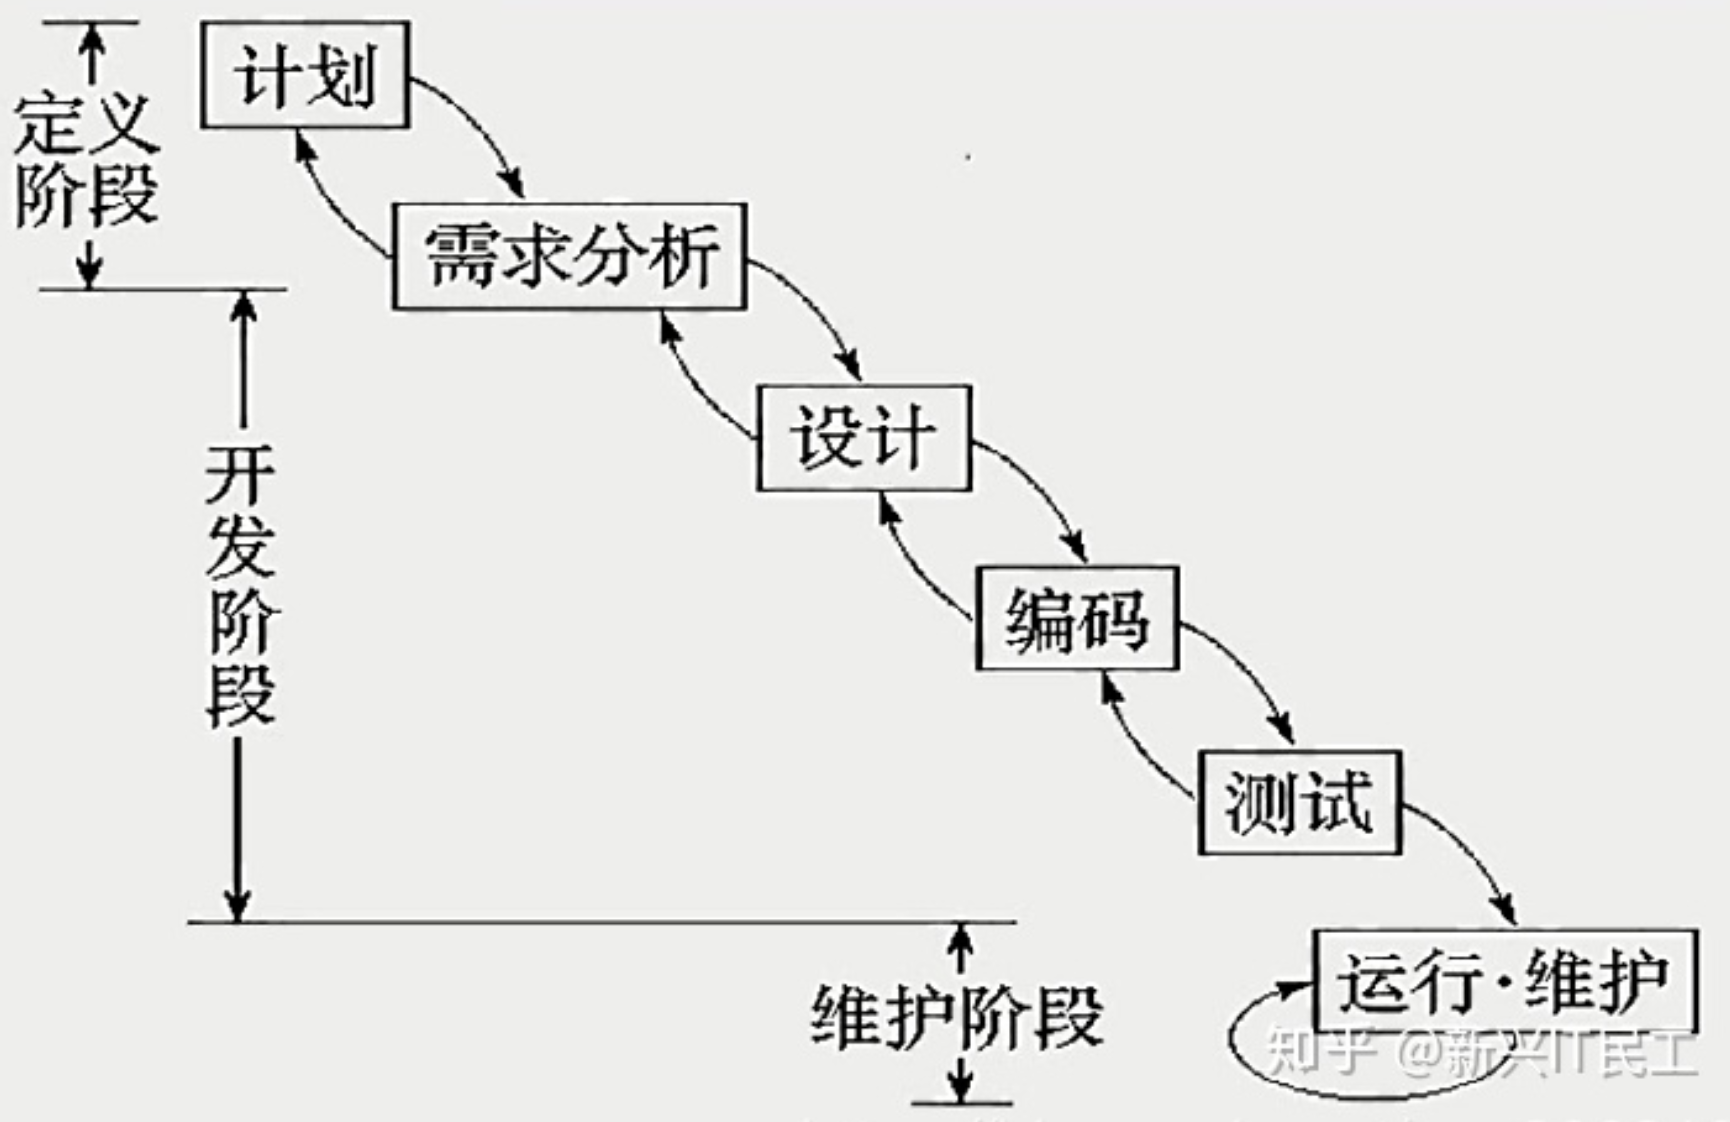
\includegraphics[width=.6\textwidth]{fig/DevOps_WaterFall.png}
\end{figure}

瀑布模型为了保证整个软件可控,从而保证软件产品质量,对每个阶段进行管控,只有前一个阶段的输出稳定和质量过关后,才能进入下一个阶段。

这种模型在需求量相对简单和少的情况下,可以做到可控。但是随着社会的发展,各行各业对软件的依赖越来越大,各种复杂的业务都需要有软件的介入,复杂的业务场景,更短的开发周期,更频繁的业务场景变更,导致瀑布模型的开发模式无法保证有效和高质量的产品开发。因此我们需要有更好更适合的开发模型。

\subsection{迭代模型}
最简单的,我们采用分而治之的方法,将整个软件需求拆分成若干个子集,将整个过程拆分成若干个迭代,每个迭代挑选出若干子集采用瀑布模型的方式进行开发。称之为迭代模型。
\begin{figure}[H]
    \centering
    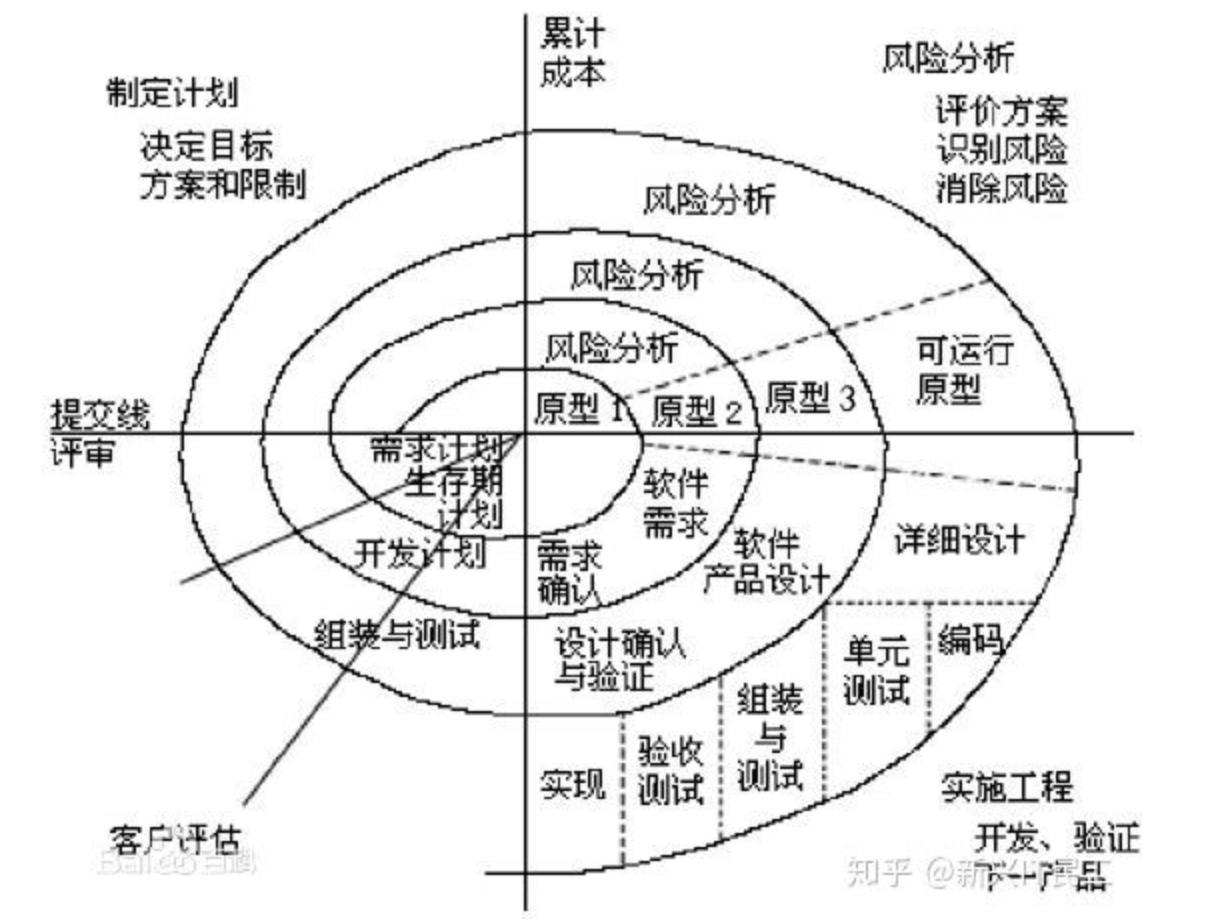
\includegraphics[width=.6\textwidth]{fig/DevOps_Iteration.png}
\end{figure}

这样,可以保证在每个迭代开发周期中,形成一个可交付的产品子集,逐步增量的进行交付。

理论上讲,通过控制迭代的需求范围,迭代开发可以适用大多数软件开发场景了。但是随着互联网和移动业务的崛起,对于软件的更新/构建速度提出了前所未有的要求。在迭代开发中,每个迭代还是走的需求设计/概要设计/详细设计/开发/测试/部署的流程。一旦一个迭代的范围和时间确定,为保证质量,原则上是不调整需求的。而一个迭代的流程下来,少说一个月两个月的。但是在移动互联网时代,为了快速响应用户需求来占领市场,需求是不断变化的,根本没有可能等待一个迭代结束之后再重新调整需求。因此,面向用户需求的软件开发理念就迅速在业界流行起来,也就是敏捷开发。

\subsection{敏捷开发}
我们来看一下敏捷开发的定义,引用百度百科上的定义:敏捷软件开发(英语:Agile software development),又称敏捷开发,是一种从1990年代开始逐渐引起广泛关注的新型软件开发方法,是一种能应对快速变化需求的软件开发能力。它们的具体名称、理念、过程、术语都不尽相同,相对于“非敏捷”,更强调程序员团队与业务专家之间的紧密协作、面对面的沟通(认为比书面的文档更有效)、频繁交付新的软件版本、紧凑而自我组织型的团队、能够很好地适应需求变化的代码编写和团队组织方法,也更注重软件开发过程中人的作用。

我个人对这个定义的理解是敏捷开发是一套方法论,为了适应频繁变化的需求而产生的。而在软件开发流程上相对于上述的瀑布和传统迭代模型而言,\textbf{最关键的变化就是从面向书面的文档转变为面向人员合作}。在前述的流程中,\textbf{强调的是每个阶段的可靠性},只有当每个阶段的输出完成后才进入下一个阶段(包括文档输出,文档也会作为一个重要的输出,成为下一阶段的输入)。\textbf{而敏捷开发更强调的是人与人之间的合作和沟通,而不是依赖文档}(当然,不是不需要文档,必要的文档记录是很重要和必要的工作)。为了保持足够有效的人员沟通,团队的规模就不可能很大。因此就只能是小而精的团队,通过有效的沟通快速将需求实现。从而小步快跑的进行快速迭代。

上面是一个敏捷开发的一个方法论,不是一个具体的实现方法,一个比较著名的方法就是scrum。

而在快速迭代的过程中,每个需求和阶段的重点是通过人员之间的合作来推动,而人总是没有机器和工具的可靠(也就是说,人总是会犯错),为了保证质量和流程的稳定,一系列的工具被开发出来,这些工具也成为了敏捷开发的一部分。

因此,我理解的\textbf{敏捷开发应该是一套实现了方法论的实践 + 工具集合}。

敏捷开发与瀑布式开发的对比图:
\begin{figure}[H]
    \centering
    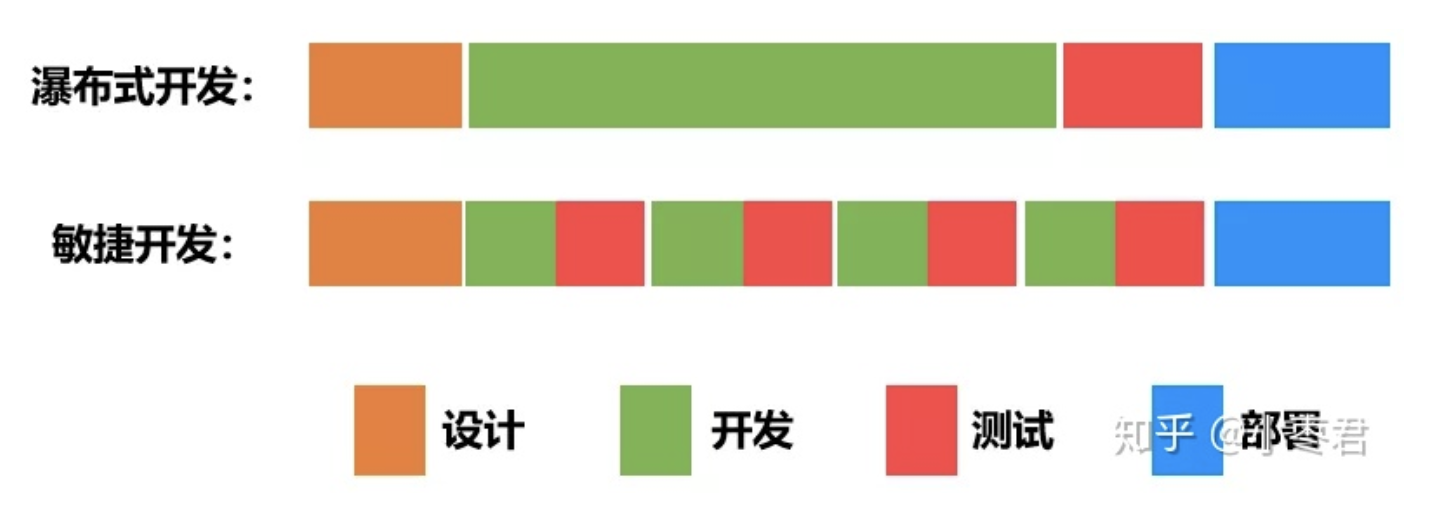
\includegraphics[width=.6\textwidth]{fig/DevOps_Agile_vs_Waterfall_1.png}
\end{figure}

敏捷开发大幅提高了开发团队的工作效率,让版本的更新速度变得更快。很多人可能会觉得,“更新版本的速度快了,风险不是更大了吗?”

其实,事实并非如此。敏捷开发可以帮助更快地发现问题,产品被更快地交付到用户手中,团队可以更快地得到用户的反馈,从而进行更快地响应。而且,DevOps小步快跑的形式带来的版本变化是比较小的,风险会更小(如下图所示)。即使出现问题,修复起来也会相对容易一些。
\begin{figure}[H]
    \centering
    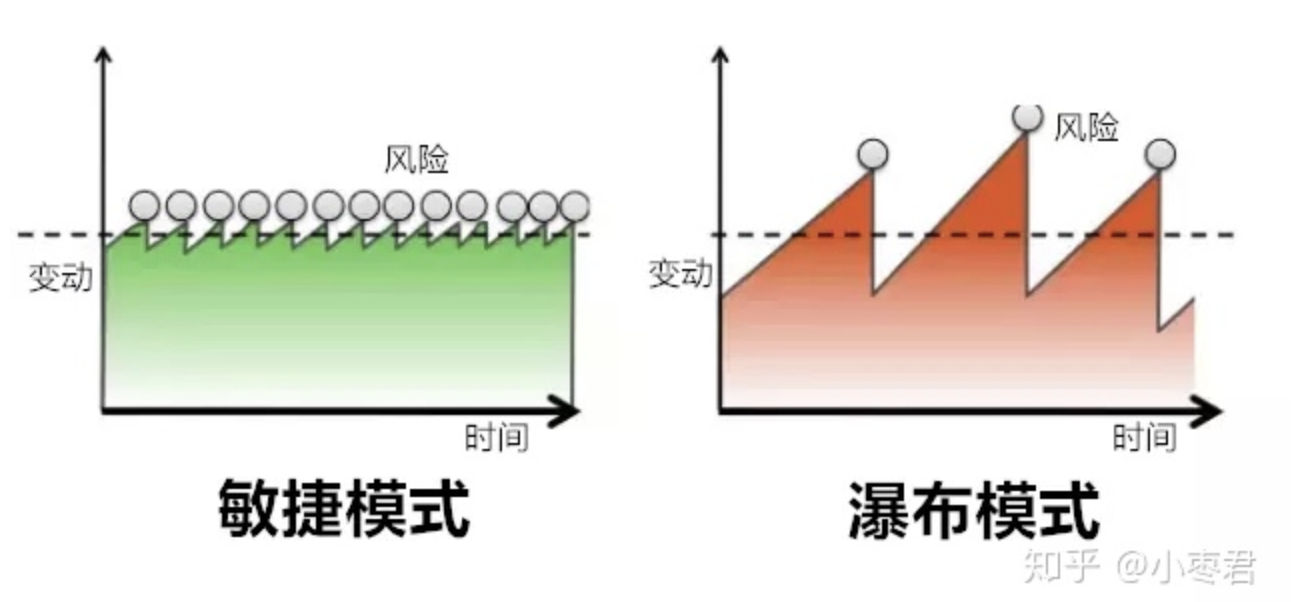
\includegraphics[width=.6\textwidth]{fig/DevOps_Agile_vs_Waterfall_2.png}
\end{figure}

虽然敏捷开发大幅提升了软件开发的效率和版本更新的速度,但是它的效果仅限于开发环节。研发们发现,运维那边,依旧是铁板一块,成为了新的瓶颈。

运维工程师,和开发工程师有着完全不同的思维逻辑。运维团队的座右铭,很简单,就是“稳定压倒一切”。运维的核心诉求,就是不出问题。

什么情况下最容易出问题?发生改变的时候最容易出问题。所以说,运维非常排斥“改变”。于是乎,矛盾就在两者之间集中爆发了。

这个时候,我们的DevOps,隆重登场了。

\section{企业软件开发流程现状}
讲到这里,就想先引入下所在企业的现状,碰到的问题及问题的思考,在这层思考的基础上去考虑DevOps的可行性和落地方法。也就是说,本人是想将DevOps作为解决方案之一来做思考的。

本人所在企业的业务是ToB的业务,和移动互联网从需求层面来讲是有很大区别的。一般来说,ToB的业务都是面向某一个特定的行业,行业属性极强,比如医疗,工业等领域,作为IT界的专业人士完全无法了解到其中的专业知识,更有甚者连最基本的常识都没有。这点和大多面向ToC的移动互联网不一样,移动互联网的业务一般都是基于常识,比如基于个人消费的电商,音乐软件等,产品经理都可以基于常识+个人体验做到对用户的引导来提出需求。这点在本人看来,对于开发流程是至关重要的,因为不管是什么样的流程,都是源自于需求,而软件本身只是一个人类生活中实现各种业务需求的工具,偏离了需求,软件也就没有存在的价值。

\subsection{逐渐暴露的问题}
上面的一大段提到的问题会衍生出下面几个关键问题:

\begin{itemize}
\setlength{\itemsep}{0pt}
\setlength{\parsep}{0pt}
\setlength{\parskip}{0pt}
    \item 我们团队在产品的需求上话语权太低。在碰到不同客户的不同需求上,对于客户的引导难度非常大。一个简单的例子就是,对于一个需求的优先级和重要性,无法有一个客观的判断,而对于客户而言,他提出的每一个需求对他而言都是重要和关键的,而我们的团队无法对其进行判别,更别说去对客户进行引导。

    \item 企业是一个初创团队,没有足够的行业经验积累。产品是基于某几家合作单位客户需求搭建起来的,是否具有业务上的普适性有待考证。

    \item 由于上述两个问题,就会造成在多个项目同时推进时,无法判断是否能由一个产品或者说时一套代码来交付

    \item ToB的业务往往是需要强可靠性和非常低的错误容忍度。简单的一个说明就是,你在发朋友圈的时候,由于程序bug导致发送失败,而且导致输入没有保存,你除了发点牢骚,心想着换个app,再默默的重新输入一次之外没有别的想法,而tob的业务可能就会导致某条流水线失败,工业事故或者更有甚者就是影响到人的生命。
\end{itemize}

因此,在实际的软件开发过程中,企业的开发模式应该是处于半敏捷开发的模式。整体来说还是需求->设计->开发->测试的模式。在产品开发初期及产品成型后的交付初期,需求相对确定,产品规模和业务复杂度较低,团队规模也不大。

\begin{itemize}
\setlength{\itemsep}{0pt}
\setlength{\parsep}{0pt}
\setlength{\parskip}{0pt}
    \item 每个迭代的时长控制在一周到两周左右。

    \item 需求文档往往就是一个截图和excel列表,在团队中通过会议进行同步和说明。
    
    \item 测试往往提前介入,及时将开发输出的需求进行测试,在过程中完善测试用例(测试的用例文档的目的往往是为了留档,进行知识储备)。让每个迭代的构建和发布时间相对缩短。
\end{itemize}

在半年到一年的交付之后,需求复杂度和代码耦合性越来越高。这个流程越来越陷入到焦油坑中:
\begin{itemize}
\setlength{\itemsep}{0pt}
\setlength{\parsep}{0pt}
\setlength{\parskip}{0pt}
    \item 需求往往要经过多次讨论,需要集合越来越多上下游的开发测试人员参与讨论,讨论的时间往往就是半天到一天。

    \item 开发代码牵一发动全身,if-else堆积如山,圈复杂度急剧上升。
    
    \item 测试很难保证测试质量,任何一个bug的修复都会导致意想不到的bug出现,根本无法提前介入测试,或者说提前介入测试基本没有起到应用的作用,在交付压力的情况下,测试会成为交付进度的牺牲品。
    
   \item 为了保证交付质量,每个环节不得不加入大量的文档和评审,保证上下游对改动的理解和范围一致。
   
   \item 到了不重构就无法推进的境地,而进度和人员规模很难保证互不影响。
\end{itemize}

可以看到,敏捷开发模式逐步退回到迭代模型中。由人员合作为导向变成了由文档为导向,每个阶段的“墙”越来越厚。

\subsection{堆积如山的环境}

一般来说,刚开始我们是规划了几套环境来保证日常的开发工作
\begin{itemize}
\setlength{\itemsep}{0pt}
\setlength{\parsep}{0pt}
\setlength{\parskip}{0pt}
    \item 本地环境:很好理解,每个开发人员的办公环境,不管是物理机还是虚拟机。用于开发人员本地调试,保证需求代码开发完成。

    \item 开发环境:开发人员维护,所有的代码提交之后,可以较为频繁和灵活的构建,作为代码的第一次整合。
    
    \item 测试环境:每个迭代规划若干次构建,每次构建后不做改动,由测试团队在此发现问题。
    
   \item 生产环境:测试确认无误后,将相应的改动部署,投入业务生产当中。
\end{itemize}

当项目越来越多时,每个项目都需要配置相同的环境。还有一些专用的环境,比如性能测试环境,为了保证稳定和演练上线步骤出现的预发布环境等等。光是环境都有一大把。虽然在现在虚拟化和容器技术的支撑下,不需要机房里堆上一大堆的物理服务器,但是对于每台虚拟机的管理也是一个相当繁琐的工作。也是影响交付效率下降的一个重要原因。

\subsection{Dev VS Ops,难以调和的矛盾}
我们的团队中没有专门负责部署和运维的团队,一般由开发或者测试的人来兼任这部分工作。但是不阻碍我们可以把这两部分工作区分开来考虑。对于已经商用的项目,规划多少需求到一个迭代中去开发和交付,是对整个团队的选择题。是尽可能多的上新的需求还是降低风险尽量少的控制需求是每次都会纠结的问题。

\begin{itemize}
\setlength{\itemsep}{0pt}
\setlength{\parsep}{0pt}
\setlength{\parskip}{0pt}
    \item 尽快的响应客户需求,将新开发的功能尽可能多的排入计划。上线失败的风险就会增加。

    \item 为了稳定尽可能少的逐步上需求,会导致客户满意度下降。
\end{itemize}

虽然没有两个团队之间的部门墙问题,同样还是存在Dev和Ops之间的矛盾。

\subsection{解决方案之一 -- DevOps}
上面说了这么一些,总的说来就是研发和交付效率随着业务和代码的复杂度上升而显著下降,就需要有更好的流程和工具来解决这样的问题。自然而然的,团队就将注意力放到了大火的DevOps上。

DevOps的维基百科定义是这样的:

DevOps是一组过程、方法与系统的统称,用于促进\textbf{开发、技术运营和质量保障(QA)部门之间的沟通、协作与整合}。

\begin{figure}[H]
    \centering
    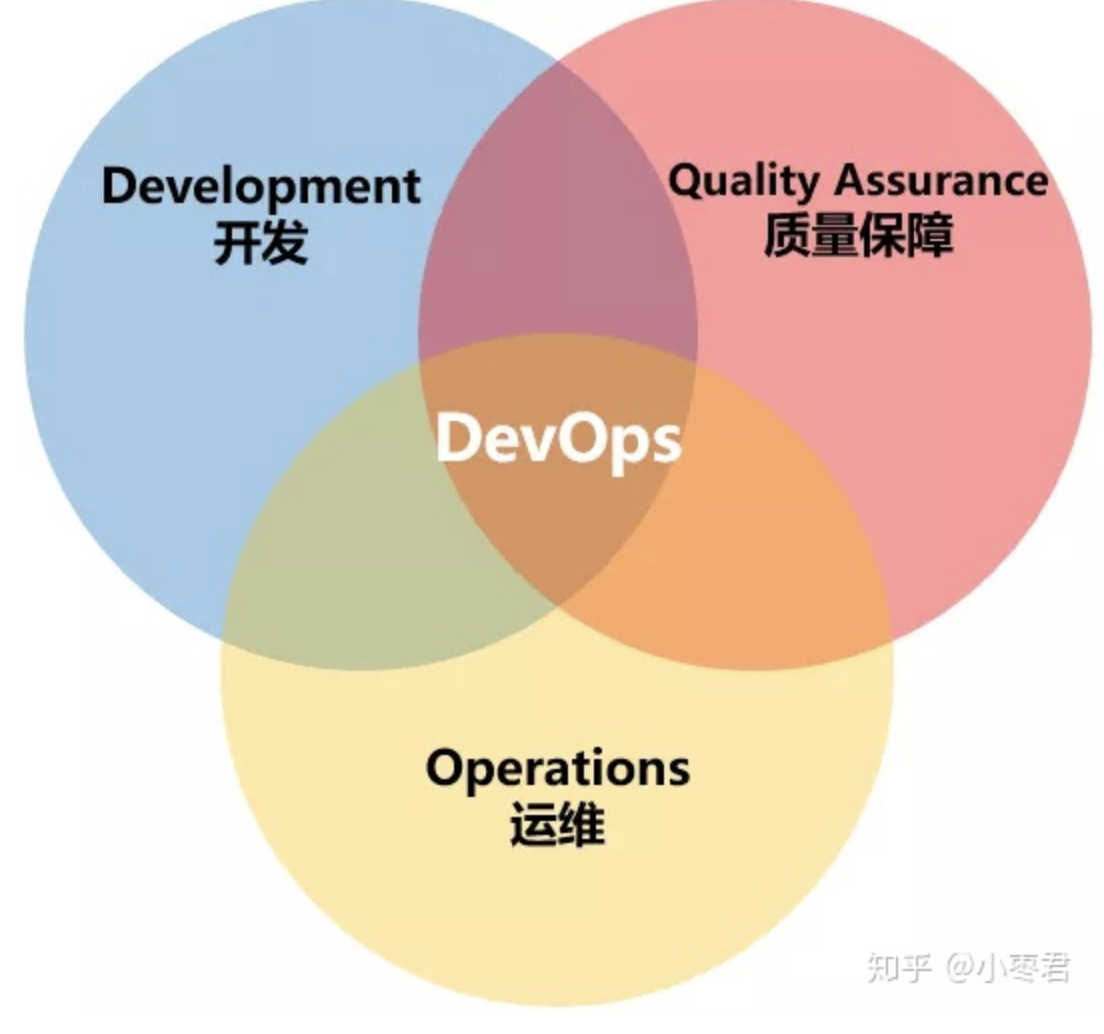
\includegraphics[width=.4\textwidth]{fig/DevOps_Dev_QA_Op.png}
\end{figure}

从目标来看,DevOps就是让开发人员和运维人员更好地沟通合作,通过自动化流程来使得软件整体过程更加快捷和可靠。

\begin{framed}
很多人可能觉得,所谓DevOps,不就是Dev+Ops嘛,把两个团队合并,或者将运维划归开发,不就完事了嘛,简单粗暴。

注意,这个观点是不对的。这也是DevOps这些年一直难以落地的主要原因。

想要将DevOps真正落地,首先第一点,是思维转变,也就是“洗脑”。不仅是运维的要洗,开发的也要洗。员工要洗,领导更要洗。

DevOps并不仅仅是组织架构变革,更是企业文化和思想观念的变革。如果不能改变观念,即使将员工放在一起,也不会产生火花。

除了洗脑之外,就是根据DevOps思想重新梳理全流程的规范和标准。

在DevOps的流程下,\textbf{运维人员会在项目开发期间就介入到开发过程中,了解开发人员使用的系统架构和技术路线,从而制定适当的运维方案}。而开发人员也会在运维的初期参与到系统部署中,并提供系统部署的优化建议。

DevOps的实施,促进开发和运维人员的沟通,增进彼此的理(gan)解(qing)。
\end{framed}

是否要用DevOps,不是因为别人用了,我们就要用。首先想了解下DevOps是什么,能解决什么问题,和现在的方式方法有什么区别,然后才能对症下药。

在敏捷开发中,已经将整个软件开发流程中的 需求->开发->测试三个环节囊括在内,指导这三个阶段的相关团队提升效率。

\begin{figure}[H]
    \centering
    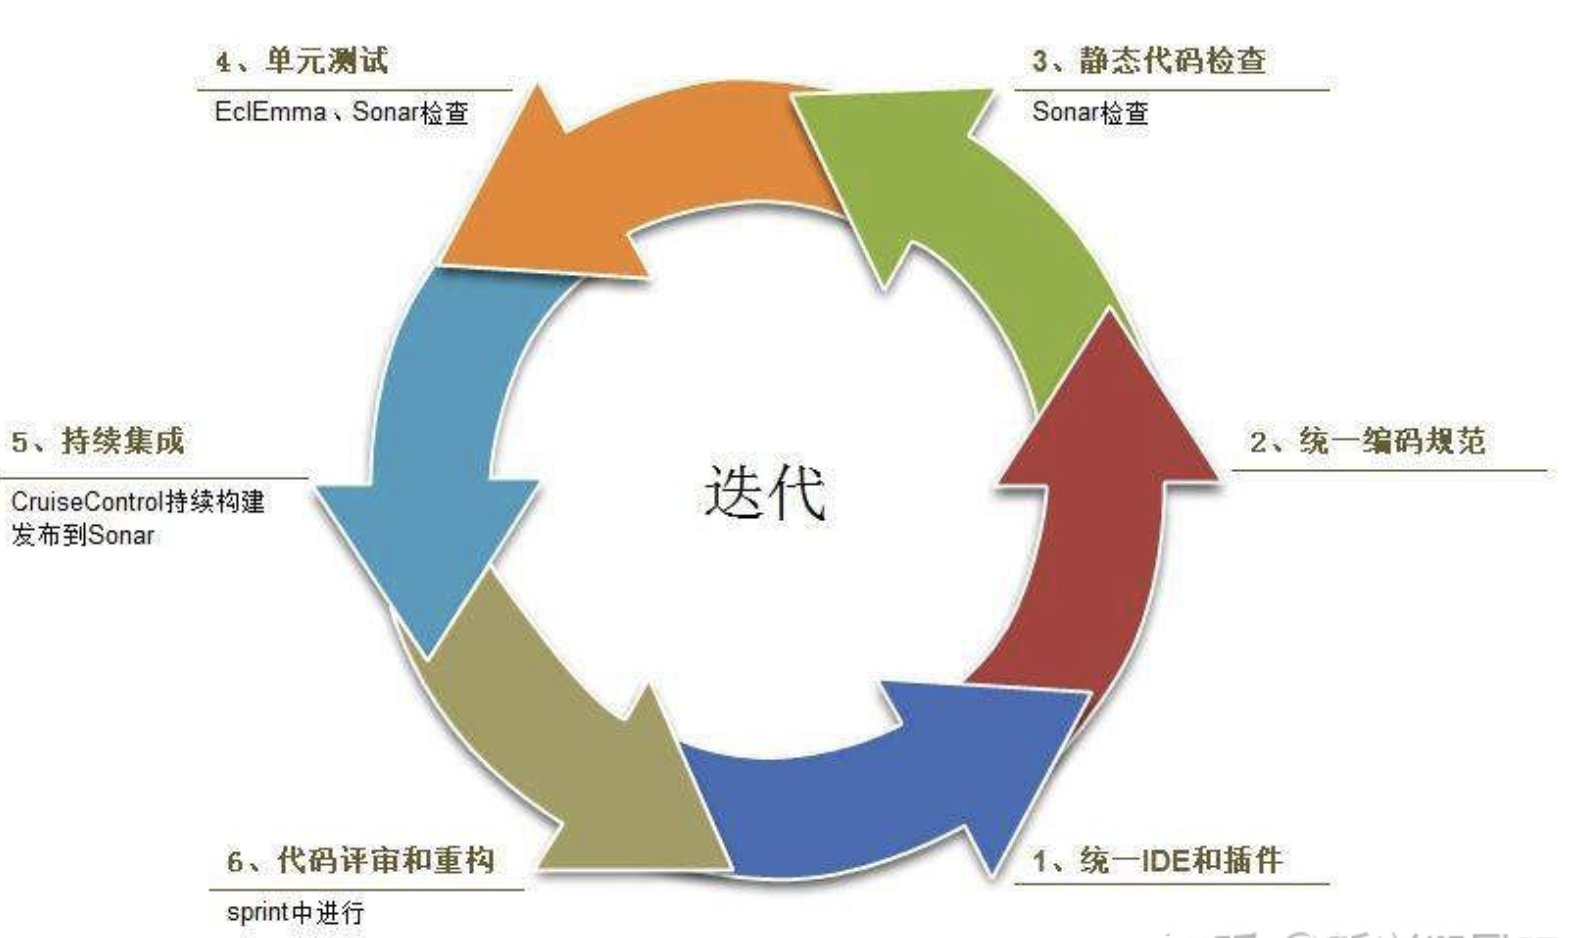
\includegraphics[width=.6\textwidth]{fig/DevOps_Lean.png}
\end{figure}

从上述的图中看到,在整个软件生命周期中的最后一个环节:部署没有被囊括进去,也就是你前面玩的再High,对于部署团队而言,输出件都是不被信任的(指输出质量,不带我玩,为啥要信你,你说啥就是啥?)。而DevOps就是想把最后这个环节也囊括到这个大循环中。

\begin{figure}[H]
    \centering
    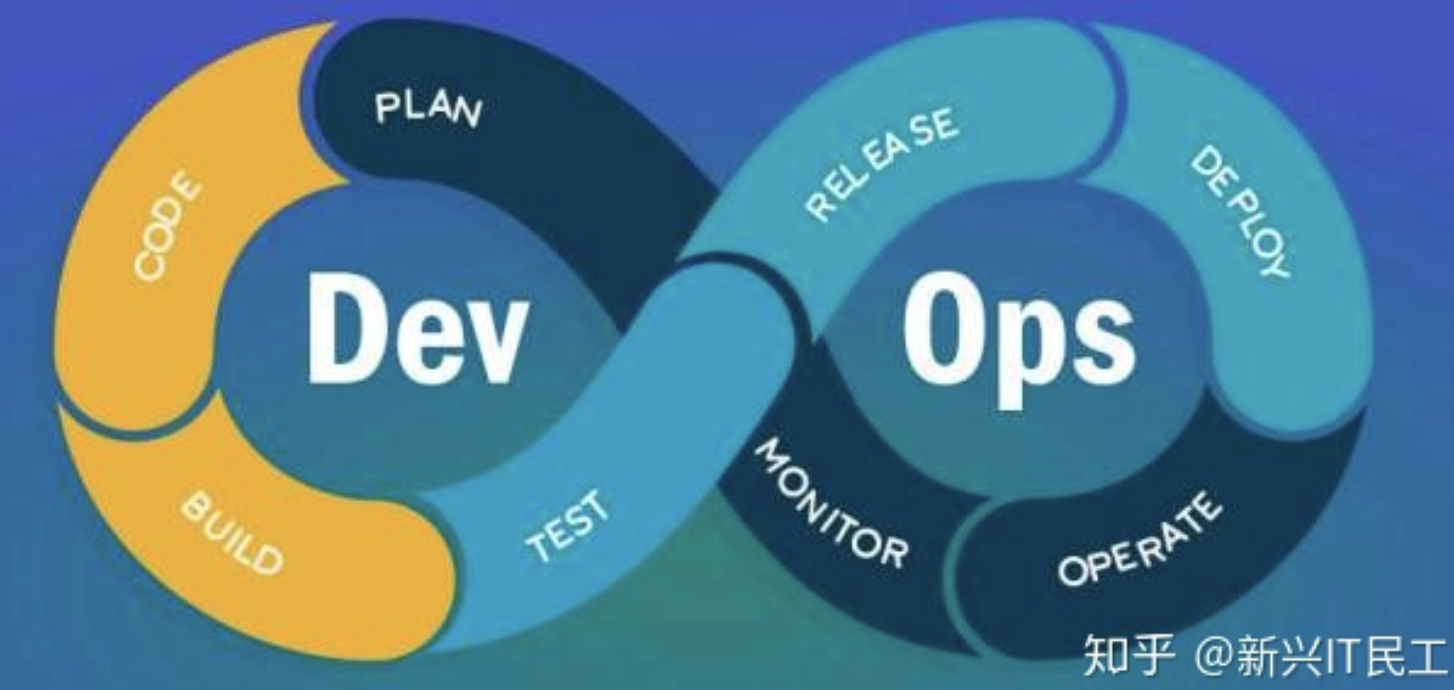
\includegraphics[width=.6\textwidth]{fig/DevOps_Lean_DevOps.png}
\end{figure}

\textbf{最终的目的是想让在这个循环中的各个阶段团队都对整个产品和整个交付过程负责,而不是只对某个阶段负责}。

回到文章的最开头,DevOps的定义里提到用的是一系列的工程方法和工具来提高效率。也就是说,用工具使得这个循环能顺利的转起来,并且要自动化的运转起来,在保证质量的前提下再越转越快。

\section{DevOps的实践方式}
上面提到了当前的几个问题:
\begin{itemize}
\setlength{\itemsep}{0pt}
\setlength{\parsep}{0pt}
\setlength{\parskip}{0pt}
    \item 业务/代码复杂度高,任何修改无法评估,失败风险大。逐步退化成靠文档去规范每个阶段。

    \item 环境多,需要大量的人力成本来维护。
    
    \item 需求开发速度和稳定性之间的矛盾。
\end{itemize}


那么就考虑下DevOps提供了哪些方法和工具来解决这些问题,从网上盗了一张图,是每个阶段的工具集合(侵删):
\begin{figure}[H]
    \centering
    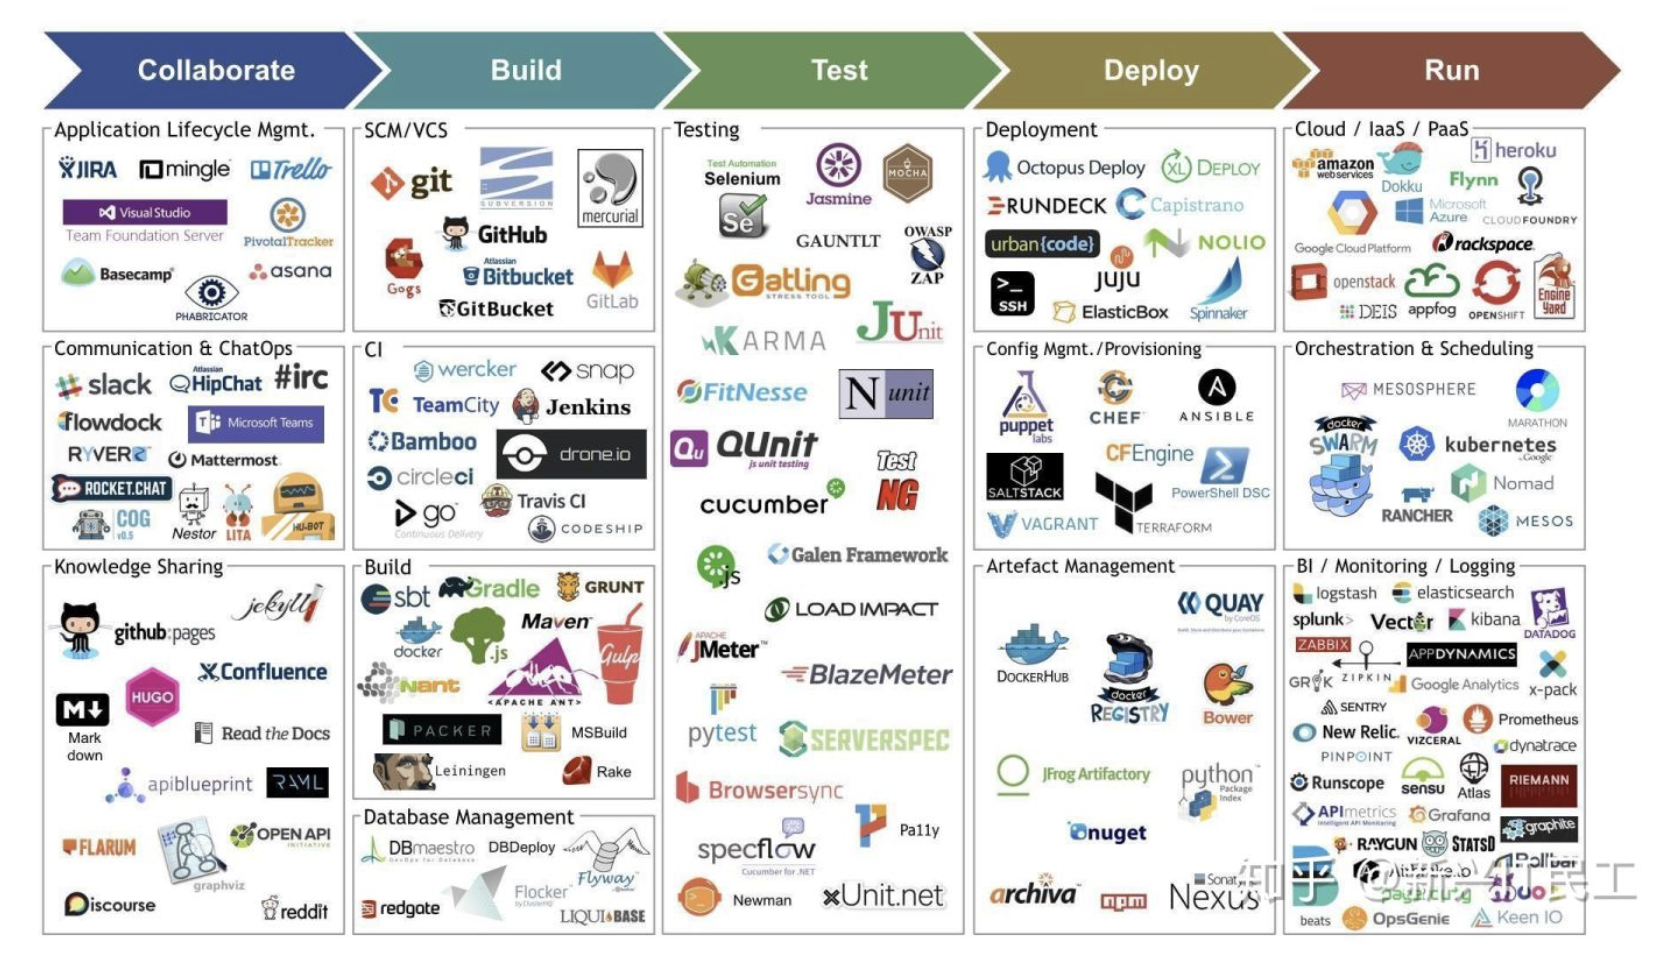
\includegraphics[width=.6\textwidth]{fig/DevOps_Tools.png}
\end{figure}

看完了简直是一脑壳包,所以要梳理下。是否引入一个新的工具或者方法的时候,总要有一个判断标准,根据数字化的标准去判断是否由于当前的方法和工具。对于研发效率这个方向而言,有下面几个指标可以参考:
\begin{itemize}
\setlength{\itemsep}{0pt}
\setlength{\parsep}{0pt}
\setlength{\parskip}{0pt}
    \item 部署频率:指应用和服务向生产环境部署代码的频率。

    \item 变更前置时间:指代码从提交到成功运行在生产环境的时长。
    
    \item 服务恢复时间:指线上应用和服务出现故障到恢复运行的时长。

    \item 变更失败率:指应用和服务在生产环境部署失败或者部署后导致服务降级的比例。
\end{itemize}

或者说,我们就是要从这想办法提高这几个指标。

或者从软件工程的角度理解,我们可以把往DevOps演进可以逐步分成下面几个阶段:

\begin{itemize}
\setlength{\itemsep}{0pt}
\setlength{\parsep}{0pt}
\setlength{\parskip}{0pt}
    \item 持续集成,代码统一管理,持续构建,开发持续输出到测试。

    \item 持续发布,持续测试,完成到产品发布的持续输出。
    
    \item 持续部署/交付,完成产品到生产环境上的持续输出。
\end{itemize}

也就是说,我认为提高效率的过程中(不管是不是DevOps),都是可以针对性的去提高这几个指标,逐步的演进到下一个阶段。在这个过程中来针对性的选择工具。使用工具就是想让各个流程步骤自动化,避免对人的依赖。

\begin{itemize}
\setlength{\itemsep}{0pt}
\setlength{\parsep}{0pt}
\setlength{\parskip}{0pt}
    \item 开发自动化,主要从配置管理,代码托管(Git),代码评审(GitHub),代码静态检查(sonar),单元测试(JUnit),配合Jenkins工具来提高。

    \item 测试自动化,引入自动化测试。
    
    \item 运维自动化,引入环境监控(Portainer),日志收集等工具。
\end{itemize}

具体的工具介绍就不写了,这个不是本篇文章的重点。策略就是发现瓶颈,解决瓶颈。发现人工部分,考虑工具来替代人工操作,不断循环往复的过程。实际上,这里必须摆脱“器”或者“术”的思路,而要采用“道”的思路:

\begin{itemize}
\setlength{\itemsep}{0pt}
\setlength{\parsep}{0pt}
\setlength{\parskip}{0pt}
    \item 不仅仅限于某种工具,再通过工具去解决某些问题。而应该是反过来的,发现了什么问题,可以用什么样的方法去解决这个瓶颈问题,再去找相关的工具。

    \item 解决问题不一定要采用某种流行的工具,不是他用了你就好用的,别人通过这个工具解决的问题,你不一定能通过这个工具解决问题,一定要从实际场景和应用出发。举个简单的例子,我们的一个产品想做日志收集,第一反应就是使用ELK + ES的方案。调研之后发现ELK的资源占用比我们产品本身的资源占用还大,ELK + ES的集群设置比产品本身的设置还困难。如果这样选型的话就是本末倒置了。而仔细分析之后我们仅仅是想将各个组件和服务之间产生的生产日志收集到一起而已,可能一个简单的SHELL脚本就可以收集了。
    
    \item 在这样的一个思路的指导下,不是使用了DevOps这个链条上的工具就表示我们是一个DevOps实践的团队了,而是团队在不停的解决瓶颈,不断提高自动化效率之后,促进了研发效率,提高了人员合作效率,我就可以说团队已经走在DevOps的康庄大道了。
\end{itemize}

\section{DevOps是一种态度和文化}
绝大多数提到DevOps的文章都会提到,\textbf{DevOps包含了两个部分,工具和文化}。换言之,\textbf{DevOps考验的不仅是一家企业的技术,更是管理水平和企业文化}。上面已经针对工具做了一个简单的思考总结。现在来谈谈文化。

对比前面所说的瀑布式开发和敏捷开发,我们可以明显看出,DevOps贯穿了软件全生命周期,而不仅限于开发阶段。

\begin{figure}[H]
    \centering
    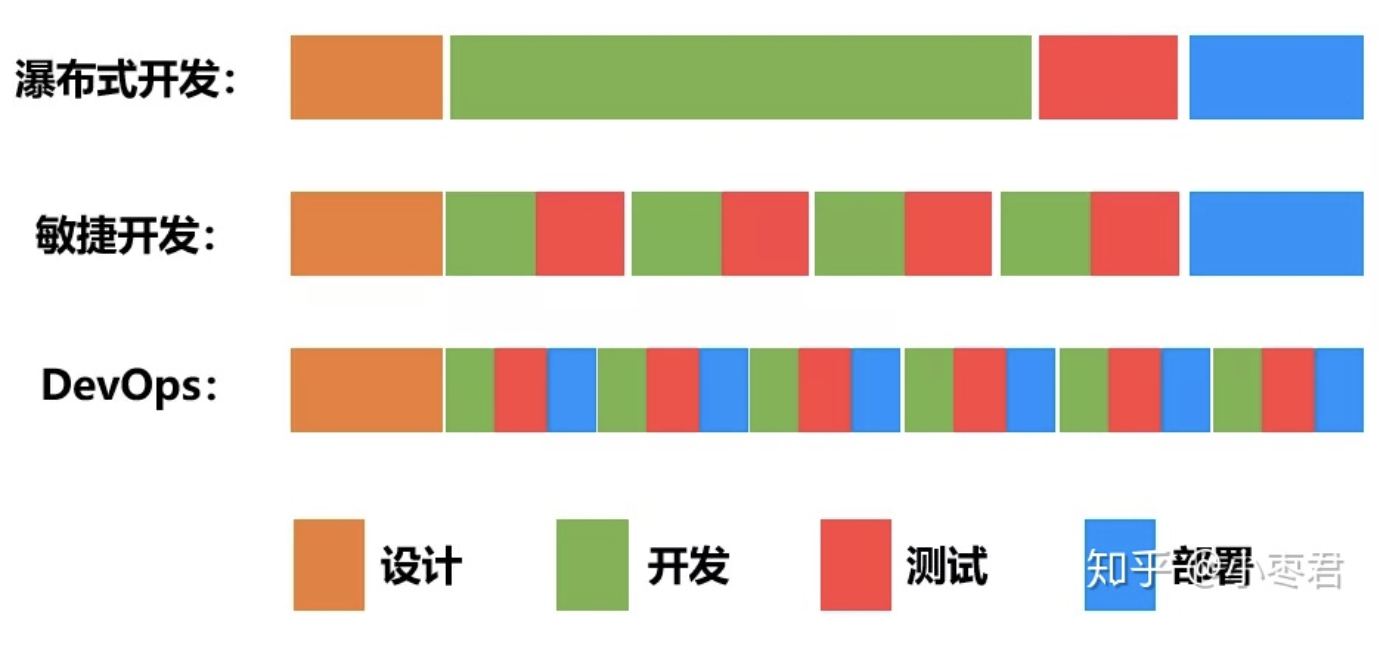
\includegraphics[width=.6\textwidth]{fig/DevOps_Waterfall_vs_Agile_vs_DevOps.png}
\end{figure}

下面这张图,更明显地说明了DevOps所处的位置,还有它的价值:

\begin{figure}[H]
    \centering
    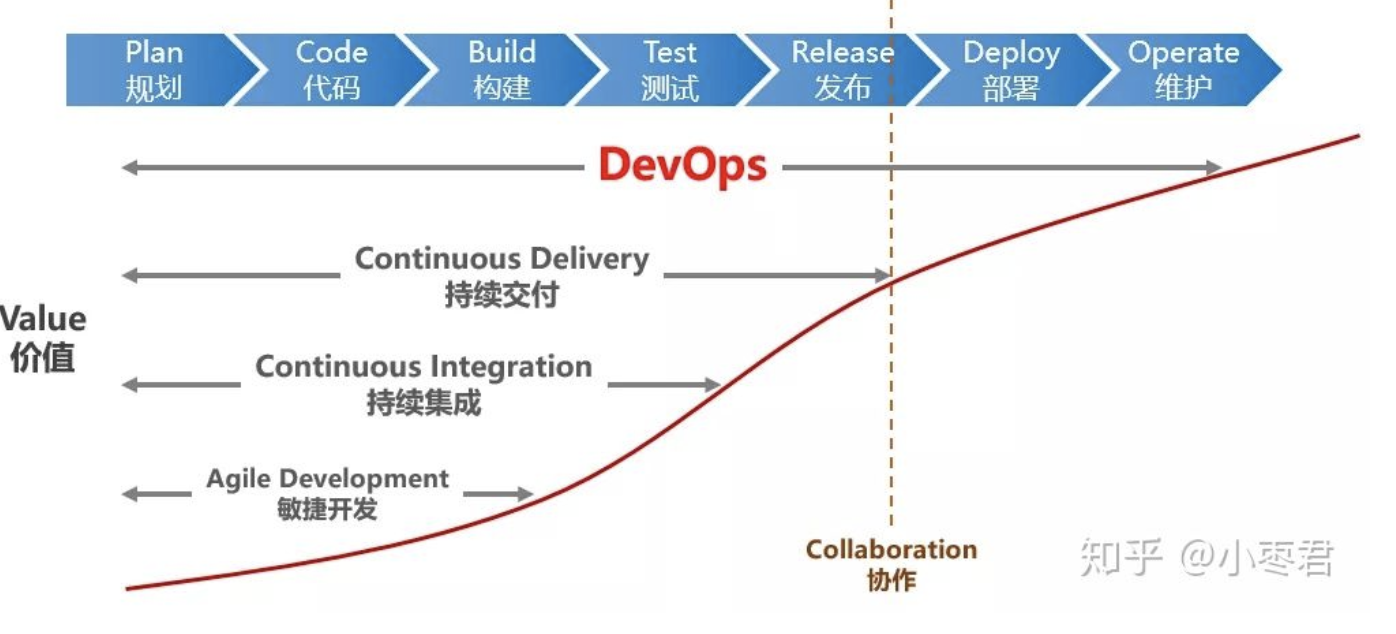
\includegraphics[width=.6\textwidth]{fig/DevOps_Value.png}
\end{figure}

本人在另外一篇文章 【管理】IT公司管理团队结构思考 提到了:企业文化就是一群人的做事风格,或者说是在做选择题,做决策的一种指导思想。而DevOps就是想提供一种有效的选择和指导思想。
\begin{itemize}
\setlength{\itemsep}{0pt}
\setlength{\parsep}{0pt}
\setlength{\parskip}{0pt}
    \item 统一目标而不是分割目标,DevOps的目的是想让整个软件开发生命周期中的所有环节都对结果负责,这里的结果是整体、业务或者商业上的结果,而不是割裂成若干个小环节的局部结果。而术业有专攻,每个阶段肯定是由若干个专业团队负责的,在管理流程上很容易的将每个团队分开管理考核,很容易导致团队之间的对立。因此需要在管理流程上对这个目标进行合理的引导(制度上),而不是去阻碍这种态度的形成。

    \item 预防大于治疗,基于上面一点,负责每个阶段的团队都需要多走出一步,向前一步,向后一步。这样才能弥补每个环节之间的间隙。而不是等到上一个环节出了问题之后再去返回去修改,这时追责的意义实际上已经不大。因此必须整个团队达成一致,是要主动迈出一步,而不是事后追责。才能形成一个有效的循环。
    
    \item 拥抱变化,软件开发是一个变化巨大的行业,需求、技术、甚至是人员本身都在快速的变化中,因此持续改进是应对变化的最有效的办法。快速发现问题,再快速解决问题。在团队统一目标,每个环节伸出左右手拉住上下游,形成一个车轮迅速往前推进。

    \item 另外,我想说下我理解的全栈工程师,不是一个人通吃整个开发的生命周期,当然刚开始可能是需要有几个一专多能的牛人构建出产品的雏形。但是只有融合不同的专才的团队才能让整个开发生命周期更长久,更稳定。而全栈指的是在目标统一的前提下,利用全局的思路去指导每个环节的研发工作。

    \item 很多人讨论是文化先行还是工具先行的问题,本人认为这不是一个串行关系,工具是一个自底向上的过程,在持续改进中积累。而文化需要一个自顶向下的过程,在演进到某个阶段,需要取得企业管理层的一致后,在公司导向,制度制定等方面向下推广。两个方向同时发展,才能取得比较好的效果。
\end{itemize}

最后,引用网络上的一句话,文化 = 人 + 流程 来做一个小小的总结。


%\printbibliography
\bibliography{../ref}
\bibliographystyle{IEEEtran}
\end{document}